\section{Conclusioni}

\subsection{Informazioni aggiuntive}
Per comprendere meglio alcune scelte che hanno influenzato
l'implementazione della soluzione, \`e necessario fornire alcune
informazioni aggiuntive.
\subsubsection{Invio dell'ordine}
L'invio di un ordine \`e stato realizzato tramite una pagina HTML che
implementa a tutti gli effetti un form. L'utente sceglie la tipologia di
ordine da inviare. Selezionata la tipologia, l'ordine viene inviato al
sistema, mentre all'``utente'' compare una schermata che conferma
l'avvenuto invio. \\\\
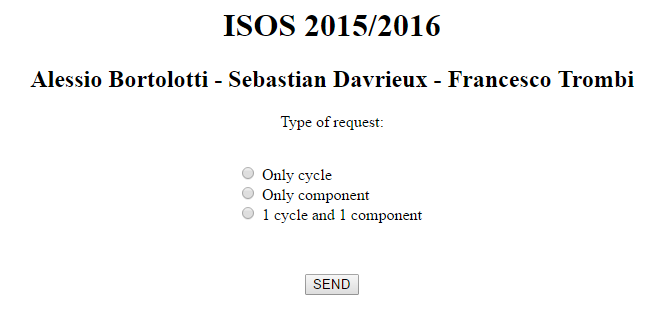
\includegraphics[scale=0.7]{immagini/formOrder.png}\\

\includegraphics[scale=0.7]{immagini/formConfirmation.png}\\
\subsubsection{Avvio del sistema}
Per implementare con semplicit\`a l'avvio del sistema, si \`e scelto di
scrivere un file {\tt .bat}, che permette tramite il suo avvio di
lanciare tutti i servizi Jolie.
\subsubsection{Camunda + WildFly}
La versione di Camunda utilizzata per l'implementazione della soluzione
\`e quella che comprende WildFly, a causa di una migliore conoscenza del
software.

\subsection{Problemi riscontrati}
Durante l'implementazione della soluzione sono comparsi alcuni problemi.
\subsubsection{Messaggi da e per l'utente}
Il messaggio di avvio del processo \`e stato implementato senza alcuna
difficolt\`a: i problemi sono sorti nel momento in cui si deve
manipolare un dialogo attivo. In quel caso un evento intermedio deve
interagire con un messaggio da parte dell'utente genera un errore, nel
quale il sistema non trova nessuna componente ``in ascolto'' di tale
messaggio.
\subsubsection{Bug generazione del WSDL}
Durante la generazione dei file WSDL, effettuata tramite il tool
{\tt jolie2wsdl}, si \`e riscontrato un problema: i file WSDL così
generati non erano infatti validi per il tool {\tt wsdl2java},
necessario per permettere l'interfacciamento tra il sistema implementato
in Camunda ed i servizi implementati in Jolie.
Per valutare il problema, si \`e deciso di effettuare alcuni test
tramite il software SoapUI, riscontrando che in questo caso i file WSDL
venivano accettati; ma, nel momento in cui venivano utilizzati per
eseguire alcune chiamate, Jolie rispondeva segnalando un errore di
mismatch tra tipi.
Il problema \`e stato risolto scrivendo i file WSDL a mano.

%\subsection{TODO}
%\begin{itemize}
  %\item implementare secondo magazzino secondario
  %\item correggere bpmn signavio
  %\item controllare descrizione delle parti della relazione nell'introduzione
  %\item implementazione magazzini da sistemare dopo l'aggiunta del secondo magazzino secondario
%\end {itemize}
